\item \defpoints{10} [Linear Regression and Classification]

(a) When we talk about linear regression, what does `linear' regard to? \defpoints{2}

(b) Assume that there are $n$ given training examples $\{(x_1, y_1), (x_2, y_2), \cdots, (x_n, y_n)\}$, where each input data point $x_i$ has $m$ real valued features. When $m > n$, the linear regression model is equivalent to solving an under-determined system of linear equations $\mathbf{y} = \mathbf{X}\beta$. One popular way to estimate $\beta$ is to consider the so-called ridge regression:
$$\argmin_{\beta} ||\mathbf{y}-\mathbf{X}\mathbf{\beta}||_2^2 + \lambda||\beta||_2^2$$
for some $\lambda > 0$. This is also known as Tikhonov regularization. Show that the optimal solution $\beta^*$ to the above optimization problem is given by
$$\mathbf{\beta}^* = (\mathbf{X}^{\top}\mathbf{X} + \lambda \mathbf{I})^{-1}\mathbf{X}^{\top}\mathbf{y}$$
Hint: You need to prove that given $\lambda>0$, $\mathbf{X}^{\top}\mathbf{X} + \lambda \mathbf{I}$ is invertible. \defpoints{5}

(c) Is the given data set linear separable? If yes, construct a linear hypothesis function to separate the given data set. If no, explain the reason. \defpoints{3}
\begin{table}[h]
    \centering
    \begin{tabular}{c|cccccc}
        Data & (1,3) & (4,4) & (3,-6) & (-2,1) & (-3,5) & (-6,-4) \\ \hline
        Label & +1 & -1 & -1 & +1 & -1 & -1
    \end{tabular}
    \label{tab:my_label}
\end{table}


\solution

(a) In linear regression, the term "linear" refers to the relationship between the parameters (coefficients) of the model and the predicted output. Specifically, a linear regression model assumes that the output is a linear combination of the input features. The model can be written as:

$$y = \beta_0 + \beta_1 x_1 + \beta_2 x_2 + ... + \beta_m x_m$$

Note that "linear" does not necessarily refer to a straight line relationship between input features and the output variable. The model can include non-linear transformations of the input features (like $x^2$, $\log(x)$, etc.), but remains linear in the parameters $\beta$.

(b) To find the optimal solution $\beta^*$ for ridge regression, we need to minimize:

$$J(\beta) = ||\mathbf{y}-\mathbf{X}\mathbf{\beta}||_2^2 + \lambda||\beta||_2^2$$

Expanding the squared norms:
$$J(\beta) = (\mathbf{y}-\mathbf{X}\mathbf{\beta})^T(\mathbf{y}-\mathbf{X}\mathbf{\beta}) + \lambda \beta^T \beta$$
$$J(\beta) = \mathbf{y}^T\mathbf{y} - 2\beta^T\mathbf{X}^T\mathbf{y} + \beta^T\mathbf{X}^T\mathbf{X}\beta + \lambda \beta^T \beta$$
$$J(\beta) = \mathbf{y}^T\mathbf{y} - 2\beta^T\mathbf{X}^T\mathbf{y} + \beta^T(\mathbf{X}^T\mathbf{X} + \lambda \mathbf{I})\beta$$

To find the minimum, we differentiate with respect to $\beta$ and set it to zero:
$$\frac{\partial J(\beta)}{\partial \beta} = -2\mathbf{X}^T\mathbf{y} + 2(\mathbf{X}^T\mathbf{X} + \lambda \mathbf{I})\beta = 0$$

Solving for $\beta$:
$$(\mathbf{X}^T\mathbf{X} + \lambda \mathbf{I})\beta = \mathbf{X}^T\mathbf{y}$$
$$\beta^* = (\mathbf{X}^T\mathbf{X} + \lambda \mathbf{I})^{-1}\mathbf{X}^T\mathbf{y}$$

Now we need to prove that $\mathbf{X}^T\mathbf{X} + \lambda \mathbf{I}$ is invertible when $\lambda > 0$.

Note that $\mathbf{X}^T\mathbf{X}$ is a symmetric positive semi-definite matrix, meaning:
- For any vector $v$, $v^T\mathbf{X}^T\mathbf{X}v = ||\mathbf{X}v||^2 \geq 0$
- If $v$ is in the null space of $\mathbf{X}$, then $\mathbf{X}v = 0$ and $v^T\mathbf{X}^T\mathbf{X}v = 0$

Now, for any non-zero vector $v$:
$v^T(\mathbf{X}^T\mathbf{X} + \lambda \mathbf{I})v = v^T\mathbf{X}^T\mathbf{X}v + \lambda v^T\mathbf{I}v = v^T\mathbf{X}^T\mathbf{X}v + \lambda ||v||^2$

Since $v^T\mathbf{X}^T\mathbf{X}v \geq 0$ and $\lambda ||v||^2 > 0$ for $v \neq 0$ and $\lambda > 0$, we have:
$v^T(\mathbf{X}^T\mathbf{X} + \lambda \mathbf{I})v > 0$ for all $v \neq 0$

Therefore, $\mathbf{X}^T\mathbf{X} + \lambda \mathbf{I}$ is positive definite and hence invertible.

(c) To determine if the given dataset is linearly separable, we need to find if there exists a linear function $f(x_1, x_2) = w_1x_1 + w_2x_2 + b$ such that:
- $f(x_1, x_2) > 0$ for points with label +1
- $f(x_1, x_2) < 0$ for points with label -1

Let's plot the points and analyze:
- Positive points: (1,3) and (-2,1)
- Negative points: (4,4), (3,-6), (-3,5), and (-6,-4)

\begin{center}
    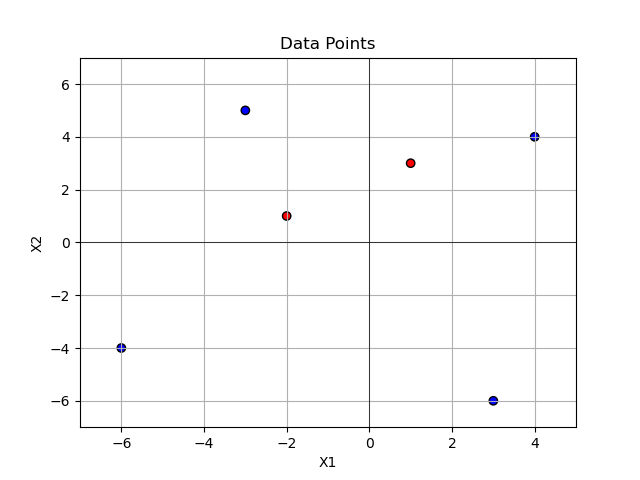
\includegraphics[width=0.5\textwidth]{figure/Figure_1.png}
\end{center}

Looking at the positions of these points, we can see that the dataset is not linearly separable. Specifically, the point (-3,5) with negative label is positioned in a way that it cannot be separated from the positive points by a single straight line without misclassifying other points.

If we try to separate the positive points (1,3) and (-2,1) from the rest, any straight line would also separate (-3,5) from the other negative points, making it impossible to correctly classify all points using a single linear boundary.

Therefore, the given dataset is not linearly separable.

\newpage